\providecommand{\main}{../../../..}
\documentclass[\main/dresen_thesis.tex]{subfiles}
\begin{document}
  \label{sec:colloidalCrystals:nanoparticle:vsm}
  \begin{figure}[tb]
    \centering
    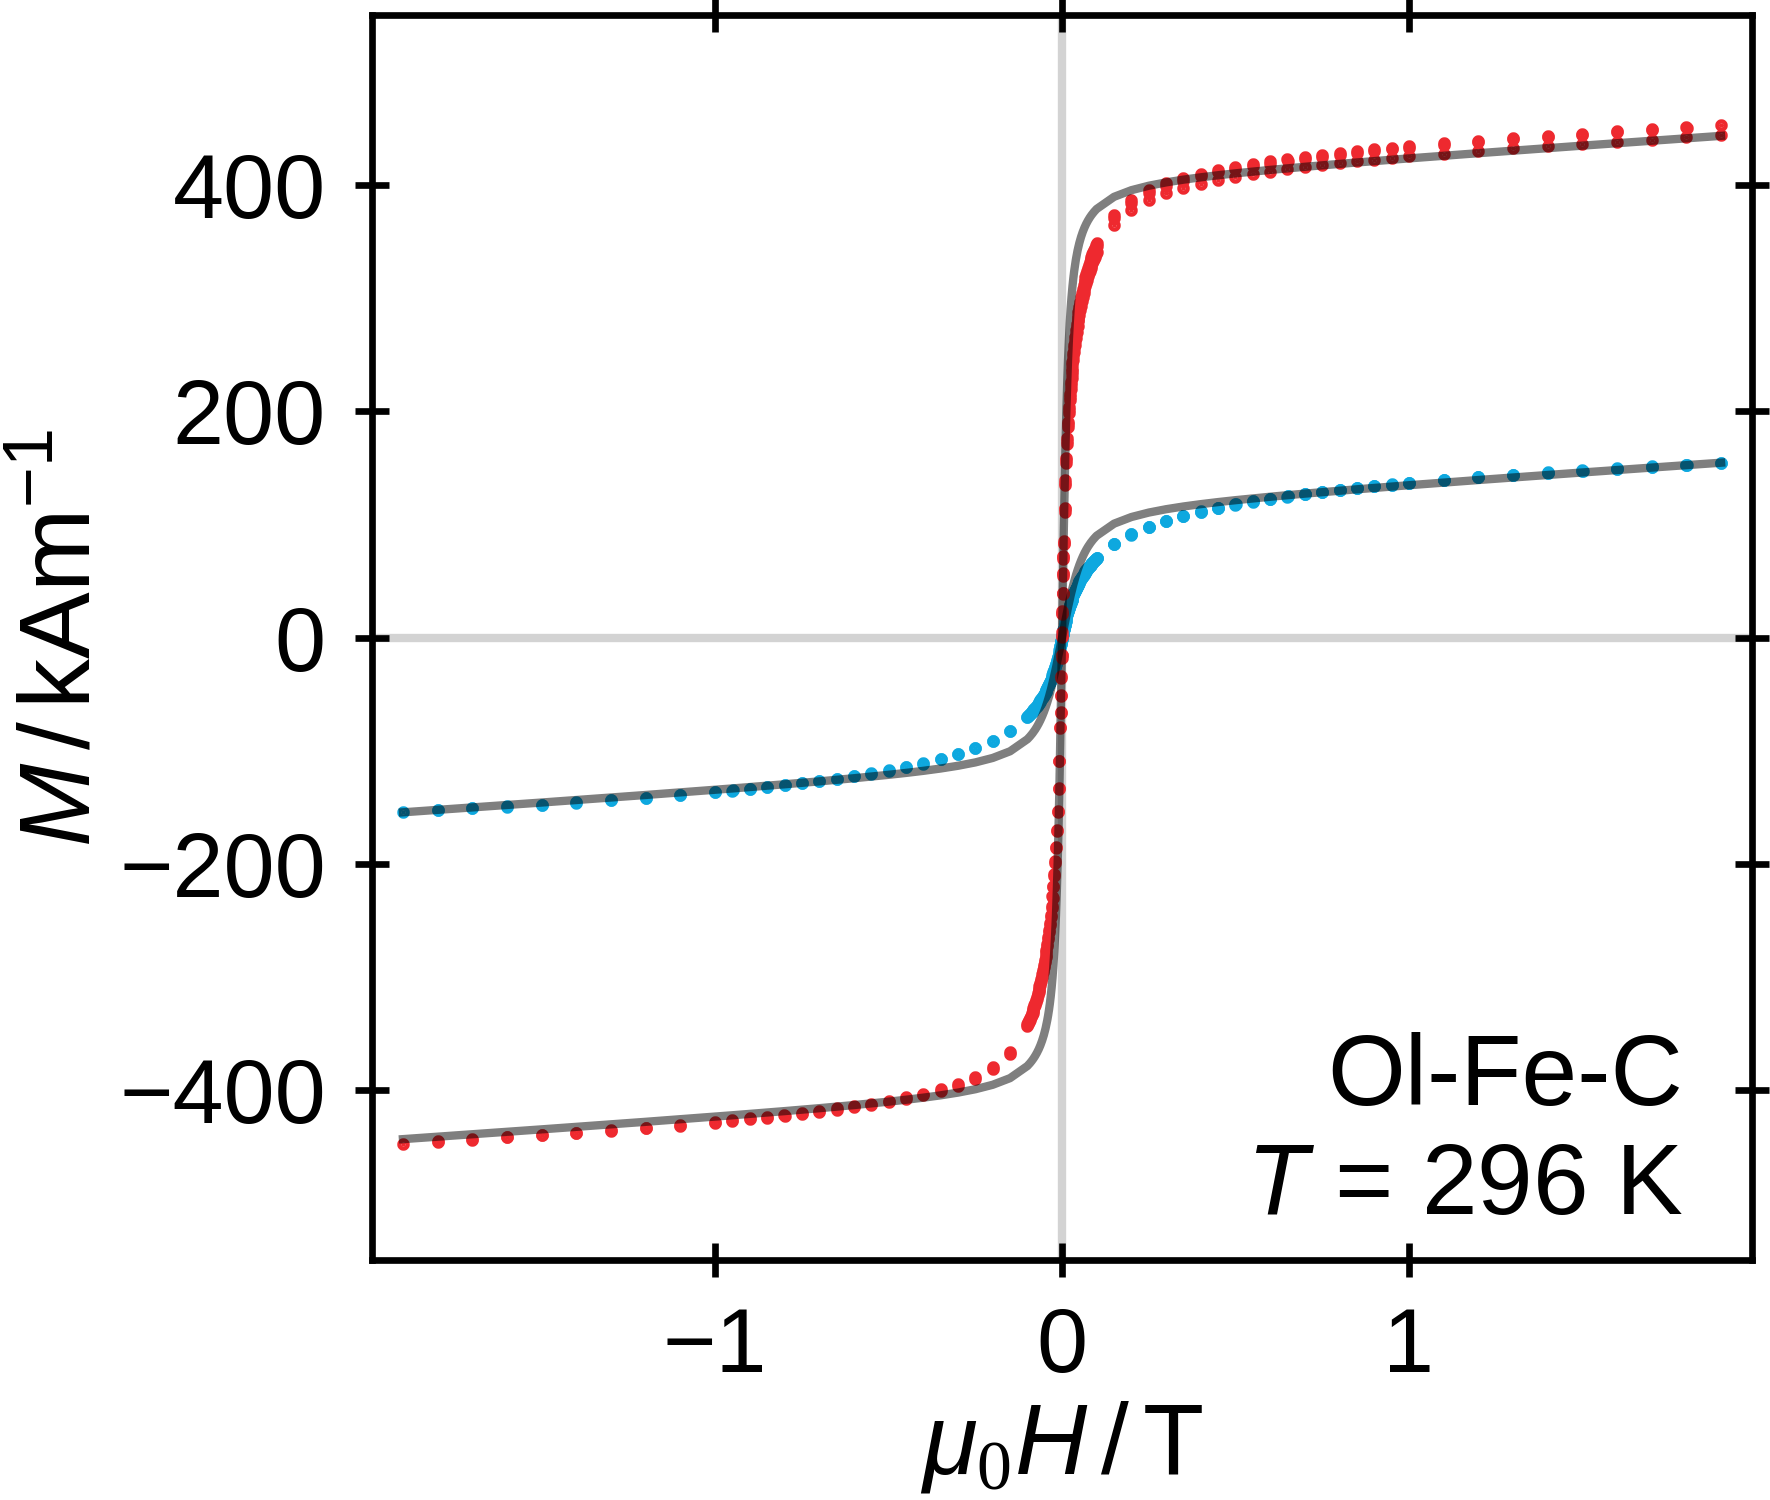
\includegraphics{colloidalCrystals_VSM_Ol_Fe_C_compare}
    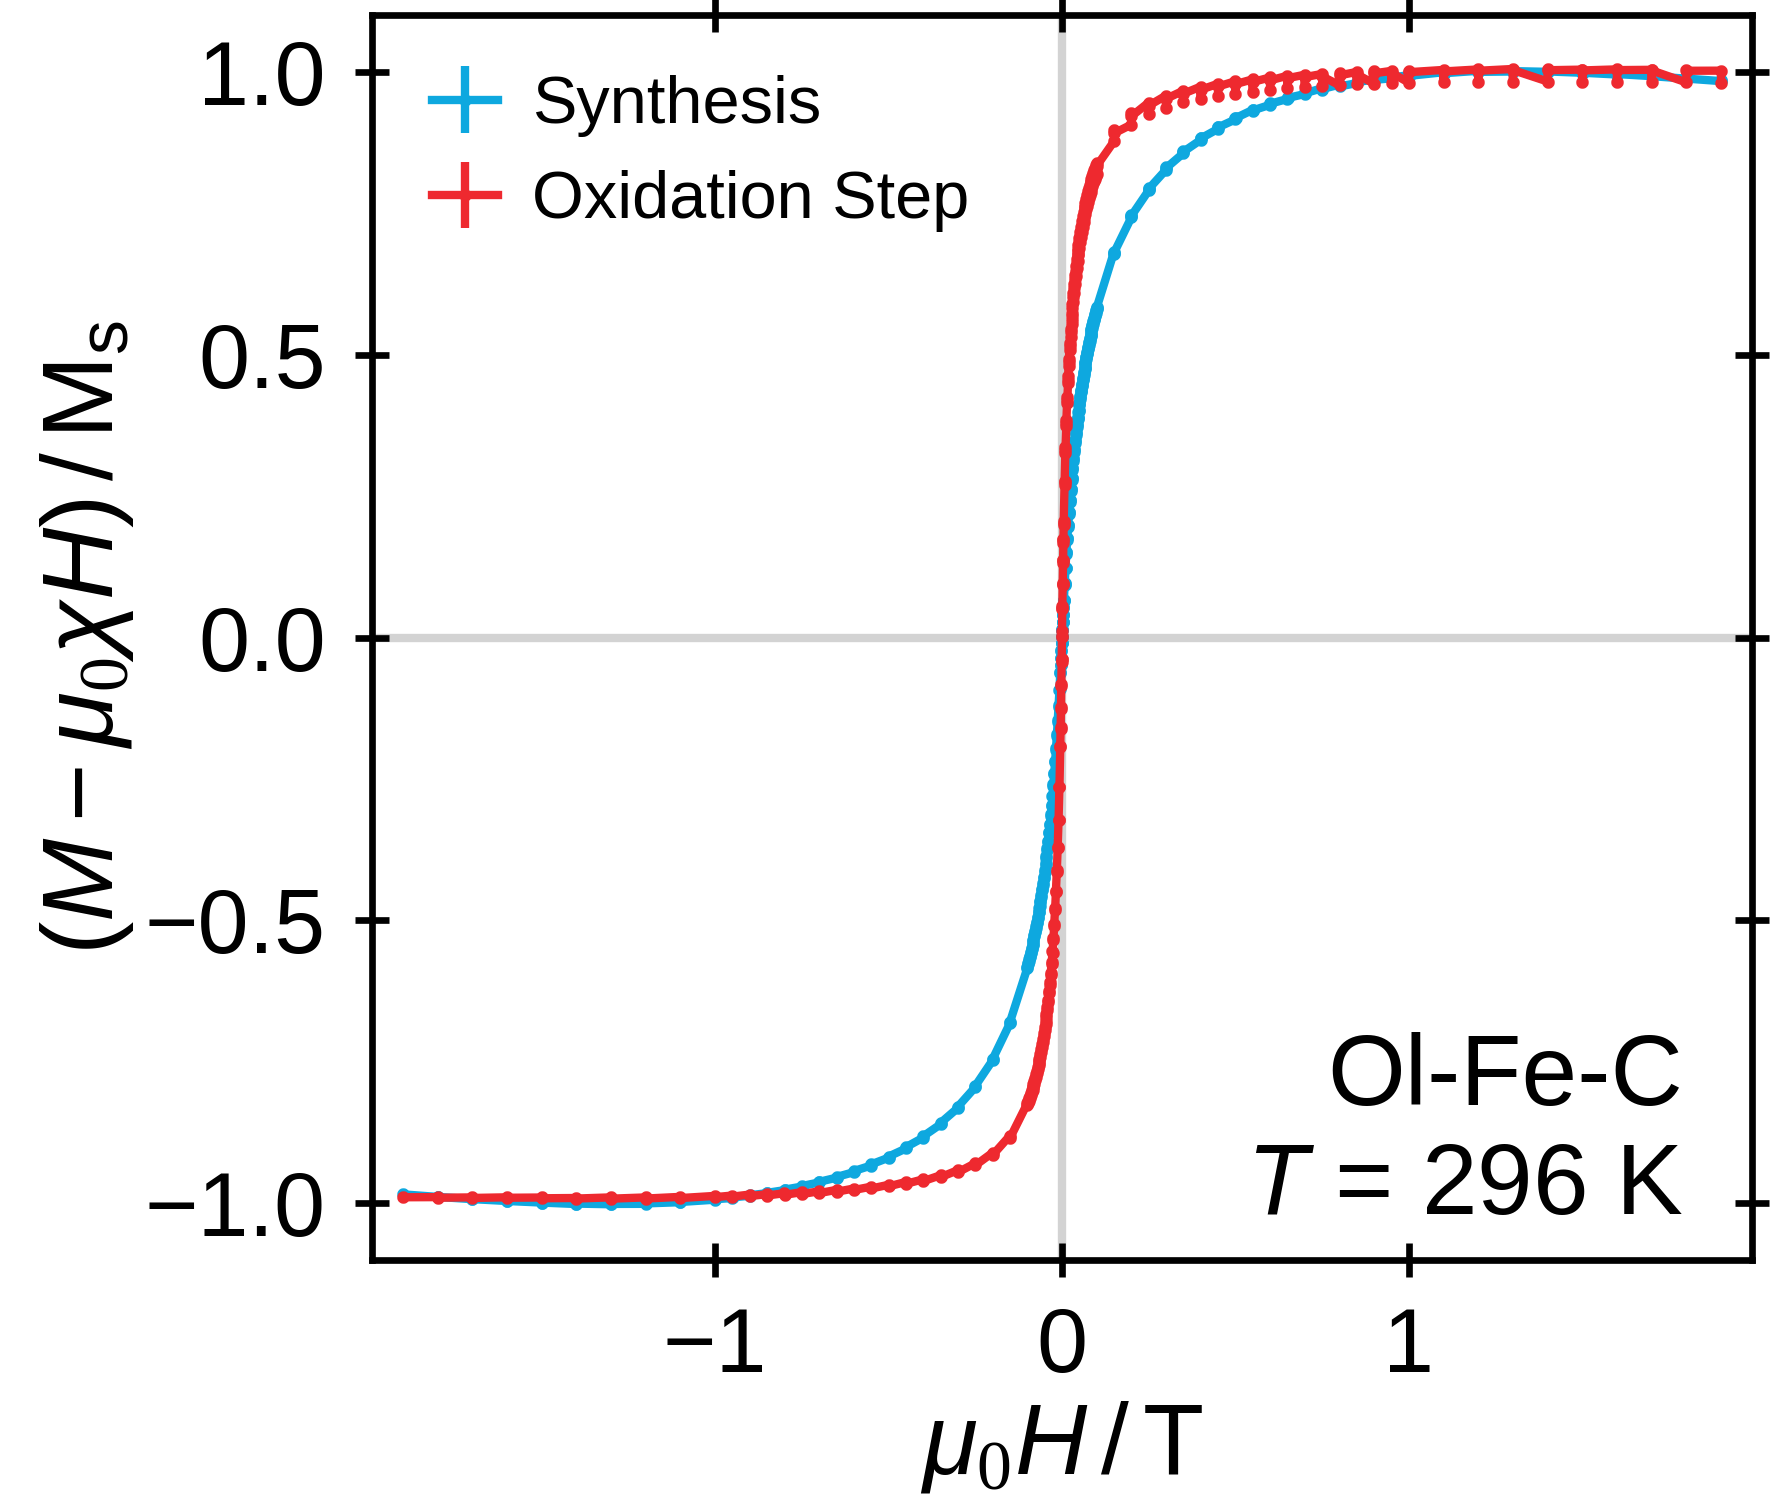
\includegraphics{colloidalCrystals_VSM_Ol_Fe_C_compareScaled}
    \caption{\label{fig:colloidalCrystals:nanoparticle:vsm}Room temperature VSM of Ol-Fe-C performed on a dry powder right after nanocube synthesis and after an additional oxidation step. The data is shown as rescaled by the magnetic moment estimated from the data at low fields (left) and scaled to it's saturation value after correcting for the excess susceptibility at high fields (right).}
  \end{figure}
  The magnetization of the nanocubes in a dry powder is shown in \reffig{fig:colloidalCrystals:nanoparticle:vsm} measured right after synthesis and after an additional oxidation step.
  The obtained data from the powder deviates from a typical Langevin behaviour with excess susceptibility.
  The solid lines show the curve expected for a Langevin behaviour, when the slope at small fields is used to determine the magnetic moment.
\end{document}
